\documentclass[
    12pt,
    a4paper,
    oneside,
    chapter=TITLE,
    section=TITLE,
    subsection=TITLE,
    subsubsection=TITLE,
    english,
    french,
    spanish,
    brazil,
    ]{abntex2}

\usepackage{lmodern}
\usepackage[T1]{fontenc}
\usepackage[utf8]{inputenc}
\usepackage{indentfirst}
\usepackage{color}
\usepackage{graphicx}
\usepackage{microtype}
\usepackage[brazilian,hyperpageref]{backref}
\usepackage[alf]{abntex2cite}

\usepackage{listings}
\usepackage{tikz}
\usetikzlibrary{shapes, arrows}

\renewcommand{\backrefpagesname}{Citado na(s) página(s):~}
\renewcommand{\backref}{}
\renewcommand*{\backrefalt}[4]{
    \ifcase #1
        Nenhuma citação no texto.
    \or
        Citado na página #2.
    \else
        Citado #1 vezes nas páginas #2.
    \fi}

\titulo{DPCM}
\autor{DDLS}
\local{Campina Grande}
\data{\today}
\instituicao{
  \textbf{Statement of Work}
  \par
  Instituto Federal de Educação, Ciência e Tecnologia da Paraíba
  }
\tipotrabalho{Projeto de Pesquisa}
\preambulo{Especificação de projeto feito com objetivo de apresentar e auxiliar o desenvolvimento do mesmo, apresentado à comunidade do IFPB}

\definecolor{blue}{RGB}{41,5,195}
\makeatletter
\hypersetup{
        %pagebackref=true,
        pdftitle={\@title},
        pdfauthor={\@author},
        pdfsubject={\imprimirpreambulo},
        pdfcreator={LaTeX with abnTeX2},
        pdfkeywords={abnt}{latex}{abntex}{abntex2}{projeto de pesquisa},
        colorlinks=false,
        linkcolor=blue,
        citecolor=blue,
        filecolor=magenta,
        urlcolor=blue,
        bookmarksdepth=4
}
\makeatother

\setlength{\parindent}{1.3cm}
\setlength{\parskip}{0.2cm}

\makeindex

\lstset{
  language=python,
  basicstyle=\ttfamily\small,
  keywordstyle=\color{blue},
  stringstyle=\color{verde},
  commentstyle=\color{red},
  extendedchars=true,
  showspaces=false,
  showstringspaces=false,
  numbers=left,
  numberstyle=\tiny,
  breaklines=true,
  breakautoindent=true,
  captionpos=b,
  xleftmargin=0pt,
}

\tikzstyle{block} = [draw, fill=blue!20, rectangle, minimum height=3em, minimum width=6em]
\tikzstyle{sum} = [draw, fill=blue!20, circle, node distance=1cm]
\tikzstyle{input} = [coordinate]
\tikzstyle{output} = [coordinate]
\tikzstyle{pinstyle} = [pin edge={to-,thin,black}]

\begin{document}

\selectlanguage{brazil}
\frenchspacing 
\imprimircapa
\imprimirfolhaderosto

\pdfbookmark[0]{\contentsname}{toc}
\tableofcontents*
\cleardoublepage

\textual

\chapter{Problema}
DPCM é a sigla para Differential pulse-code modulation, basicamente é um circuíto que dá a diferença do valor de entrada n com o valor de n-1. Você deverá desenvolver o sistema se baseando na implementação e no diagrama de blocos abaixo.

\par
Implementação 1:
\begin{lstlisting}
def DPCM(a, x):
    aux = a-x

    if aux<0:
        return -aux

    return aux
\end{lstlisting}

\par
Diagrama de Blocos:

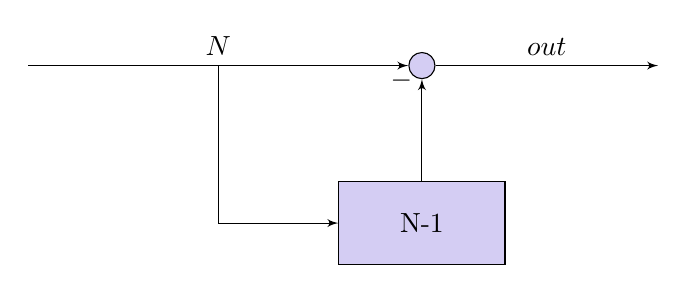
\begin{tikzpicture}[auto, node distance=2cm,>=latex']
  \node [input, name=input] {};
  \node [sum, right of=input, node distance=5cm] (sum) {};
  \node [block, below of=sum] (n-1) {N-1};
  \node [output, right of=sum, node distance=3cm] (output) {};

  \draw [->] (sum) -- node[name=OUT] {$out$} (output);

  \draw [draw,->] (input) -- node[name=N] {$N$} (sum);
  \draw [->] (N) |- (n-1);
  \draw [->] (n-1) -- node[pos=0.99] {$-$} (sum);
\end{tikzpicture}

\chapter{Interface}

A interface de comunicação do seu sistema deve atender os seguintes requisitos da \autoref{tabela-interface}:

\begin{table}[htb]
\IBGEtab{
  \caption{Especificação de Dados}
  \label{tabela-interface}
}{
  \begin{tabular}{ccc}
  \toprule
   Nome & Tipo & Tamanho em bits \\
  \midrule \midrule
   Valid & Entrada & 1 \\
  \midrule 
   DataIn & Entrada & 32 \\
  \midrule 
   Ready & Saída & 1 \\
  \midrule 
   DataOut & Saída & 32 \\
  \bottomrule
\end{tabular}
}{
  \fonte{Produzido pelos autores.}%
  \nota{Ready será levado para 1 quando o IP estiver pronto para entrada ou saída de dados.}
  \nota{Valid só será ativado quando o ready estiver levantado e servirá para a entrada de dados.}
  \nota{DataIn só será gravado quando o Valid e o Ready estiverem ativos.}
  }
\end{table}

Na \autoref{fig-maquina-estados} você pode analisar a maquina de estados do sistema.
\par
\begin{figure}[htb]
    \caption{\label{fig-maquina-estados}Maquina de Estados da Interface}
    \begin{center}
        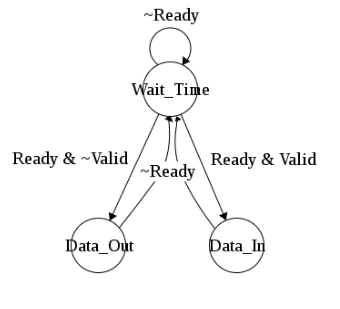
\includegraphics[scale=0.8]{imgs/maquina-estados.png}
    \end{center}
    \legend{Fonte: Produzido pelos autores.}
\end{figure}


\chapter{Estimulos}
\section{Entrada}
A entrada será uma palavra de 32 bits.
\section{Saída}
A saída deverá ser mostrada apenas quando o resultado estiver pronto e deve sair junto com a subida do ready após a entrada do número.

\section{Caso Base}
Na \autoref{fig-caso-PROJETO} temos um exemplo de como deve seu IP deve responder com os respectivos estímulos.

\begin{figure}[htb]
    \caption{\label{fig-caso-PROJETO}Caso Base do PROJETO}
    \begin{center}
        \advance\leftskip-3cm
        \includegraphics[width=\paperwidth]{imgs/caso-PROJETO.png}
    \end{center}
    \legend{Fonte: Produzido pelos autores.}
\end{figure}

\end{document}
